\definecolor{gray75}{gray}{0.75}
\newcommand{\hsp}{\hspace{20pt}}
\titleformat{\chapter}[hang]{\Huge\bfseries}{\thechapter\hsp\textcolor{gray75}{|}\hsp}{0pt}{\Huge\bfseries}
\chapter{Introduction}


In this thesis, I present the methodology behind a statistical model I created, which attempts to forecast the outcomes of and within\footnotemark{} Indian Premier League (IPL) Twenty20 (T20) cricket matches. I then test the performance of the model against two distinct benchmarks.

\footnotetext{I define the outcome of a match as simply, the team that wins the match. In contrast, an outcome within a match includes answers to questions such as: which player scored the most runs? Who took the most wickets? Which team will score the most runs in the first six overs of their innings?}

Knowledge of the game of cricket, particularly the T20 format, is assumed throughout. If the reader is unfamiliar with how the game works, a short primer can be found in \cref{chap: How Cricket Works}.

The model is trained on ball-by-ball data from the IPL's inception up to, and including the 2020 season. We test the model on predictions it makes about the 2021 season, comparing these forecasts to those from the two benchmarks. The first benchmark is historical odds from the sports betting market. I anticipate the sports markets to be a tough test for the model to overcome, especially given the decently liquid markets\footnote{More liquidity tends to translate to high accuracy/efficiency of the market.} for games in prized tournaments such as the IPL. The second benchmark we use for evaluating the model's performance is another, much simpler simulator. This has the benefit of being able to test the model's performance in areas beyond simply match outcome. With this ball-by-ball modelling approach, almost every event in the match is simulated. The results of these simulations can therefore be compared against what happened in the real world.

\section{Motivation}

The motivation behind this project comes out of sheer curiosity to see whether this type of modelling could be effective in predicting the outcome of games. When considering the problem of modelling sports more generally, my first instinct is to naively think something like, ‘how can I most authentically replicate this game, from my computer?’ I decided on the sport of cricket, given that it was clear to me that a simulator of this kind mimics the game of cricket especially well. For example, one key factor in determining the outcome of a given delivery is the specific match-up between the batter and bowler. My knowledge of the game tells me that these match-ups can have a great deal of impact on the respective probabilities for each possible outcome of that ball. A ball-by-ball simulator accounts for these possible match-ups in a way that's superior to any other approach I could think of. Before each delivery, the model will check to see who is the bowler and who is the batter, amongst other variables related to the state of the game at the time. Once these factors are known, it can sample from a distribution of probabilities, determined by these inputs. A more traditional modelling approach might take a more top-down stance. It may take team line-ups as an input and output some expected number of runs for each team across each innings as a whole. Where this approach falls short, in my opinion, is that it fails to attribute significant weight to the individual match-ups, at the heart of the game. Moreover, in the format of T20, the outcome of each individual ball, has significantly more impact on the result of the match, compared with longer formats of the game. It therefore seems appropriate to try to model the game at the most granular level we can - that of the ball.

\section{Aims of the Project}

The ultimate aim of the project is to build a model that gives accurate predictions in all areas. A ludicrously lofty ambition, I am aware. If we are able to manage that however, the possibilities for how a tool like this could be used are endless. It could guide and assist coaches in selecting optimal line-ups for their team. This includes solving problems like finding the batting order to maximise win-probability for a given match. Or answering questions such as, "how does a team's win-probability change if they sacrifice a good middle-order batter for an excellent extra bowler in their line-up?"

We could also utilise this tool in betting into the liquid IPL prediction markets when the next tournament comes around in the spring of 2022. With a model that can in theory return us probabilities for any outcome we choose, there would be no shortage of opportunities for us to bet at bookmakers and provide liquidity on the exchanges.

I know that achieving anything even remotely close to what I have just described above will be a tremendous result. I must emphasise that the point of this experiment is not to build something of the description above, but to test whether something like this \textit{can} be built.

\section{Overview of the Model}

The model that I propose can be broken down into several parts. The first is essentially a multi-class classification problem. Given there are only a finite number of possible outcomes that can happen from each ball, a probability can be assigned to each of these by the model, given a set of input parameters. A typical distribution based on frequentist probabilities across the dataset can be found in \cref{fig:intro}. Incidentally, this is the exact distribution used in the
benchmark simulator.

\begin{figure}[h]
    \centering
    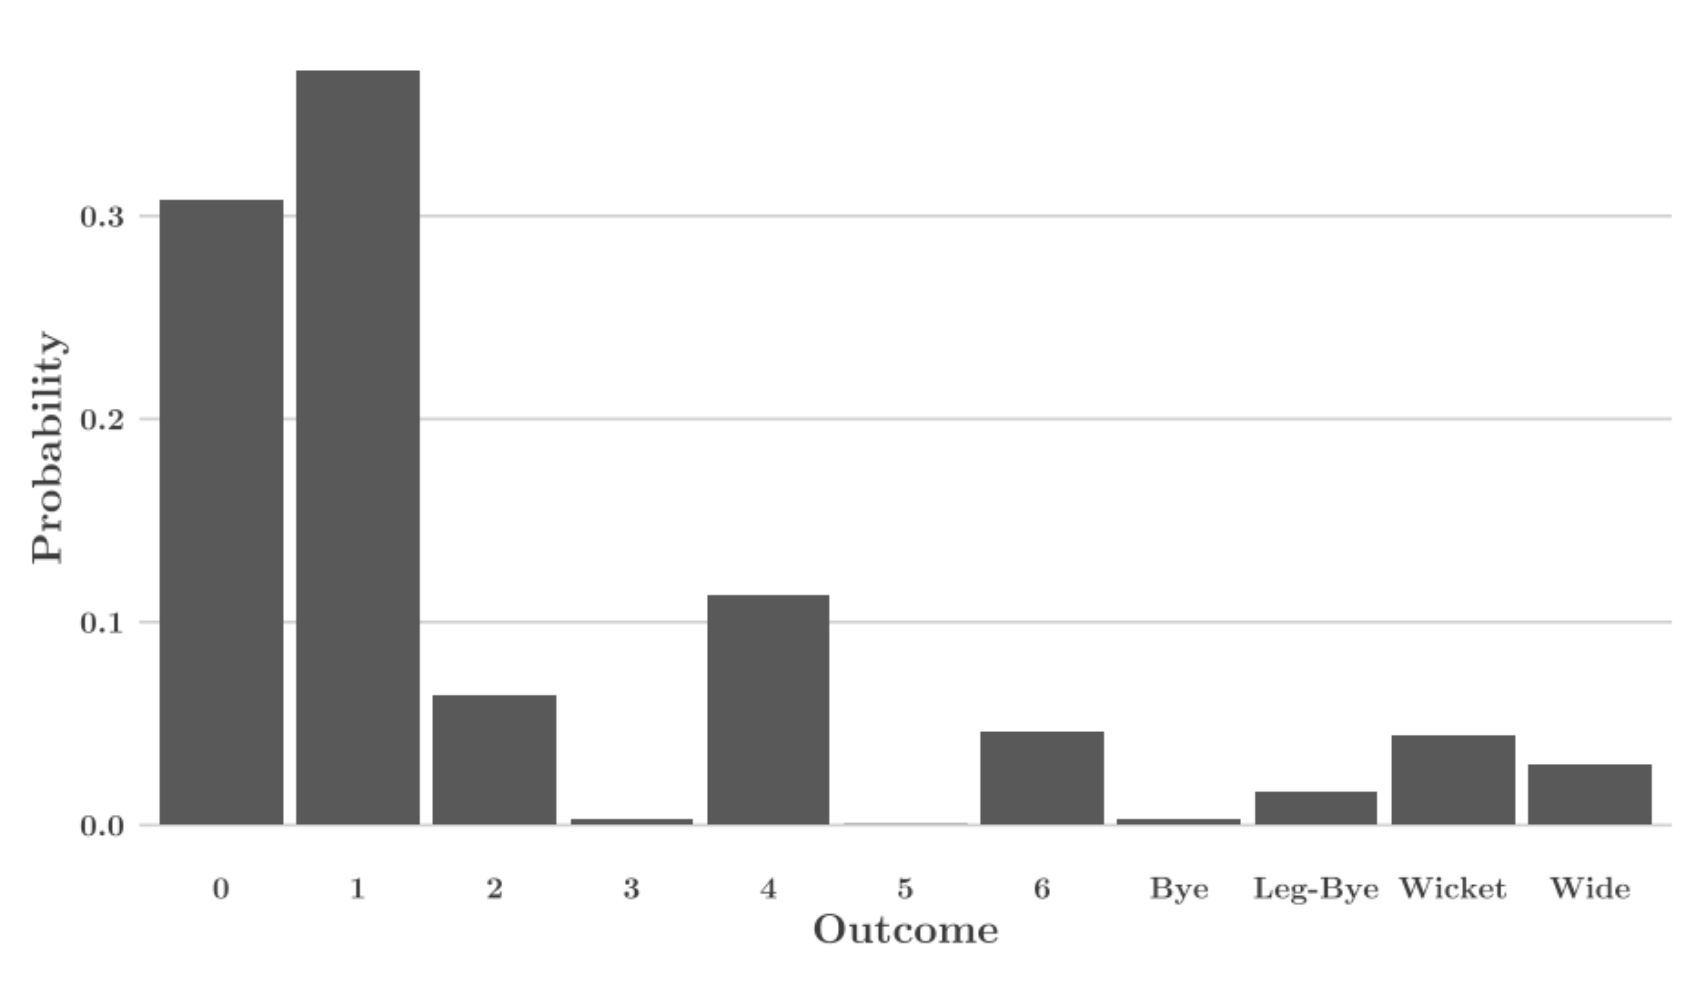
\includegraphics[width=0.75\columnwidth]{images/intro2.png}
    \caption{Showing the probability distribution of the 11 possible outcomes from a delivery.}
    \label{fig:intro}
\end{figure}

Based on which outcome gets sampled here, subsequent questions are asked, and the responses are sampled in a similarly probabilistic manner to above. For example, it is possible and not uncommon for a no-ball to be bowled by the bowler, in addition to the batsman scoring runs. This is why ‘no-ball’ is not one of the 11 initial outcomes. So if the outcome is one from zero to six runs, we sample to check for a no-ball. Run-outs are also possible in addition to runs and byes (assuming no boundary is scored) so this is checked and sampled at the end of a ‘ball’ simulation. As we’ll discover in \cref{chap: Lit}, this practice of going beyond the initial outcome sampling is a step further than what has been done before in previous experiments of this kind.